\documentclass[11pt]{article}

\usepackage[margin=1in]{geometry}
\usepackage[T1]{fontenc}
\usepackage{lmodern}
\usepackage{microtype}
\usepackage{amsmath,amssymb,amsthm,mathtools}
\usepackage{mathrsfs}
\usepackage[dvipsnames]{xcolor}
\usepackage[most]{tcolorbox}
\usepackage{graphicx}
\graphicspath{{figures/}{notes/figures/}}
\usepackage{tikz}
\usetikzlibrary{decorations.markings,patterns}
\usepackage{pgfplots}
\pgfplotsset{compat=1.18}
\usepackage{enumitem}
\usepackage{tocloft}
\usepackage[hidelinks]{hyperref}

\definecolor{courseblue}{HTML}{1F4E79}
\definecolor{lightblue}{HTML}{EAF2F8}
\definecolor{lightgreen}{HTML}{EAF7EA}
\definecolor{lightpink}{HTML}{FCE8EF}
\definecolor{lightyellow}{HTML}{FFF8D6}
\definecolor{warningyellow}{HTML}{D6A000}
\definecolor{exercisebg}{HTML}{FDEAEA}
\definecolor{exerciseframe}{HTML}{B54040}
\definecolor{examplebg}{HTML}{F4FAFE}
\definecolor{exampleframe}{HTML}{85C1E9}
\definecolor{darkgray}{HTML}{333333}
\definecolor{lightorange}{HTML}{FDEBD8}
\definecolor{orangeframe}{HTML}{E08A3C}
\definecolor{remarkbg}{HTML}{F3EEFB}
\definecolor{remarkframe}{HTML}{9B7FC9}
\definecolor{cayleyred}{HTML}{C0392B}
\definecolor{cayleygreen}{HTML}{1E8449}
\definecolor{cayleyblue}{HTML}{1F5FA0}
\definecolor{cayleyorange}{HTML}{D35400}
\definecolor{cayleypurple}{HTML}{7D3C98}
\definecolor{cayleyteal}{HTML}{117A65}

\setlength{\parindent}{0pt}
\setlength{\parskip}{0.45em}
\setlist[itemize]{topsep=0.25em,itemsep=0.15em}
\renewcommand{\cftsecleader}{\cftdotfill{\cftdotsep}}
\renewcommand{\cftsubsecleader}{\cftdotfill{\cftdotsep}}

\theoremstyle{plain}
\newtheorem{theorem}{Theorem}[section]
\newtheorem{proposition}[theorem]{Proposition}
\newtheorem{lemma}[theorem]{Lemma}
\newtheorem{corollary}[theorem]{Corollary}
\theoremstyle{definition}
\newtheorem{definition}[theorem]{Definition}
\newtheorem{example}[theorem]{Example}
\newtheorem{exercise}[theorem]{Exercise}
\newtheoremstyle{boldremark}
  {3pt}{3pt}{\normalfont}{}{\bfseries}{.}{.5em}
  {\thmname{#1}\thmnumber{ #2}\thmnote{ (#3)}}
\theoremstyle{boldremark}
\newtheorem*{remark}{Remark}
\theoremstyle{remark}
\newtheorem*{fact}{Fact}
\newtheorem*{warning}{Warning}

\tcolorboxenvironment{definition}{
  enhanced,
  unbreakable,
  colback=lightgreen,
  colframe=ForestGreen,
  boxrule=0.7pt,
  arc=2pt,
  left=6pt,
  right=6pt,
  top=5pt,
  bottom=5pt
}

\tcolorboxenvironment{remark}{
  enhanced,
  colback=remarkbg,
  colframe=remarkframe,
  before upper={\setlength{\parskip}{0.5em}},
  boxrule=0.7pt,
  arc=2pt,
  left=6pt,
  right=6pt,
  top=5pt,
  bottom=5pt
}

\tcolorboxenvironment{warning}{
  enhanced,
  colback=lightyellow,
  colframe=warningyellow,
  boxrule=0.7pt,
  arc=2pt,
  left=6pt,
  right=6pt,
  top=5pt,
  bottom=5pt
}

\tcolorboxenvironment{exercise}{
  enhanced,
  colback=exercisebg,
  colframe=exerciseframe,
  boxrule=1pt,
  arc=2pt,
  left=6pt,
  right=6pt,
  top=5pt,
  bottom=5pt
}

\tcolorboxenvironment{example}{
  enhanced,
  colback=examplebg,
  colframe=exampleframe,
  boxrule=0.7pt,
  arc=2pt,
  left=6pt,
  right=6pt,
  top=5pt,
  bottom=5pt
}

\numberwithin{equation}{section}

\newcommand{\be}{\begin{eqnarray}}
\newcommand{\ee}{\end{eqnarray}}
\newcommand{\C}{\mathbb{C}}
\newcommand{\R}{\mathbb{R}}
\newcommand{\N}{\mathbb{N}}
\newcommand{\Z}{\mathbb{Z}}
\DeclareMathOperator{\Log}{Log}
\DeclareMathOperator{\Arg}{Arg}

\DeclareMathOperator{\Hol}{\mathcal{H}\mathrm{ol}}
\DeclareMathOperator{\Real}{Re}
\DeclareMathOperator{\Imag}{Im}
\newcommand{\A}{\mathcal{A}}
\newcommand{\CT}{\C[[T]]}
\newcommand{\CLT}{\C((T))}
\tcbset{breakable}
% Compact spacing around diagrams; keep the main text at 11pt.
\newenvironment{lecturefigure}
 {\par\addvspace{0.25em}\begingroup\setlength{\parskip}{0pt}\centering}
 {\par\endgroup\addvspace{0.25em}}
\begin{document}

\begin{center}
  \colorbox{lightblue}{%
    \begin{minipage}{0.94\textwidth}
      \vspace{0.55em}
      \begin{tabular*}{\textwidth}{@{\extracolsep{\fill}}lr}
        {\color{courseblue}\bfseries\LARGE Lecture 29} &
        {\color{courseblue}\bfseries\LARGE MATH 411}\\[0.35em]
        \textbf{Fall 2026} & \textbf{Date: Nov 25, 2026}\\
        & \textbf{Instructor: Manish Patnaik}
      \end{tabular*}
      \vspace{0.45em}
    \end{minipage}}
\end{center}

\setcounter{tocdepth}{1}
\tableofcontents
\vspace{0.45em}

% Moved from the end of Lecture 28 (handwritten Lecture 27, Nov. 23).
\section{Examples of analytic isomorphisms}

Recall that in Lecture~28, we introduced the \emph{upper half-plane}
$\mathbb H=\{z\in\C:\Imag z>0\}$, the open unit disc
$D=\{z\in\C:|z|<1\}$, and the \emph{Cayley transform} $F: \mathbb H \rightarrow D$ between them. $F$ is an analytic isomorphism with inverse $G$, and they were given by the following formulas:
\[
 F(z)=\frac{i-z}{i+z},\qquad G(w)=i\frac{1-w}{1+w},
\]
Note that $F(i)=0$ (so $G(0)=i$) and we observed already that $F$ sends the real axis to the points on the unit circle with $-1$ removed: this follows from the explicit formula that for $x \in \R$, we have \[ F(x)=\frac{1-x^2}{1+x^2}+i\frac{2x}{1+x^2} \] 


To get a sense of how the Cayley transform works, consider the pictures below which trace how how $F$ acts on the boundary $\R$, on hyperbolic
geodesics (lines or semi-circles) in $\mathbb H$, and on \textit{horocycles},

\begin{lecturefigure}
\begin{minipage}{\linewidth}\centering
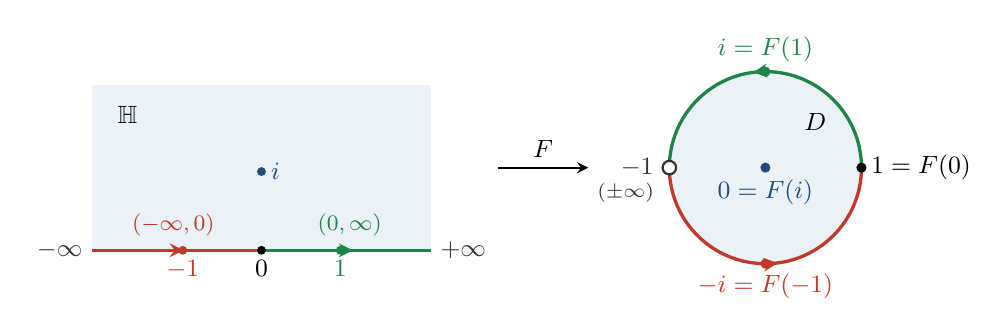
\begin{tikzpicture}[>=stealth,font=\small,
 midarrow/.style={postaction={decorate},decoration={markings,mark=at position .54 with {\arrow{>}}}}]
 % Left: upper half-plane and boundary R
 \begin{scope}[scale=1.0]
  \fill[lightblue] (-2.15,0) rectangle (2.15,2.1);
  \draw[cayleyred,very thick,midarrow] (-2.15,0) -- (0,0);
  \draw[cayleygreen,very thick,midarrow] (0,0) -- (2.15,0);
  \fill[cayleyred] (-1,0) circle (1.6pt) node[below,text=cayleyred] {$-1$};
  \fill (0,0) circle (1.6pt) node[below] {$0$};
  \fill[cayleygreen] (1,0) circle (1.6pt) node[below,text=cayleygreen] {$1$};
  \node[left,text=darkgray] at (-2.15,0) {$-\infty$};
  \node[right,text=darkgray] at (2.15,0) {$+\infty$};
  \node[text=cayleyred,font=\footnotesize] at (-1.12,0.32) {$(-\infty,0)$};
  \node[text=cayleygreen,font=\footnotesize] at (1.12,0.32) {$(0,\infty)$};
  \fill[courseblue] (0,1) circle (1.6pt) node[right,text=courseblue] {$i$};
  \node at (-1.7,1.72) {$\mathbb H$};
 \end{scope}

 % Mapping arrow
 \draw[->,thick] (3.0,1.05) -- node[above] {$F$} (4.15,1.05);

 % Right: unit disc and boundary circle
 \begin{scope}[shift={(6.4,1.05)},scale=1.22]
  \fill[lightblue] (0,0) circle (1);
  \draw[cayleygreen,very thick,midarrow] (1,0) arc[start angle=0,end angle=180,radius=1];
  \draw[cayleyred,very thick,midarrow] (-1,0) arc[start angle=180,end angle=360,radius=1];
  \fill (1,0) circle (1.5pt) node[right] {$1=F(0)$};
  \fill[cayleygreen] (0,1) circle (1.5pt) node[above,text=cayleygreen] {$i=F(1)$};
  \fill[cayleyred] (0,-1) circle (1.5pt) node[below,text=cayleyred] {$-i=F(-1)$};
  \fill[courseblue] (0,0) circle (1.5pt) node[below,yshift=-1pt,text=courseblue] {$0=F(i)$};
  \draw[darkgray,thick,fill=white] (-1,0) circle (2pt)
   node[left,xshift=-2pt,text=darkgray] {$-1$};
  \node[below left,xshift=-2pt,yshift=-2pt,text=darkgray,font=\scriptsize] at (-1,0) {$(\pm\infty)$};
  \node at (0.52,0.48) {$D$};
 \end{scope}
\end{tikzpicture}

\vspace{0.2em}
{\small\textbf{Boundary real line:} $F(x)=\frac{1-x^2}{1+x^2}+i\frac{2x}{1+x^2}$
maps $(-\infty,0)$ (red) to the lower semicircle and $(0,\infty)$ (green) to
the upper semicircle, sending $\pm\infty$ to the puncture $-1\in\partial D$.}
\end{minipage}
\end{lecturefigure}

\begin{lecturefigure}
\begin{minipage}{\linewidth}\centering
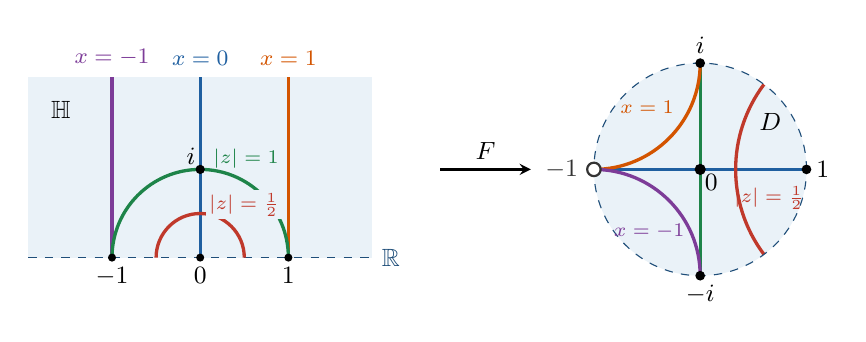
\begin{tikzpicture}[>=stealth,font=\small]
 % Left: geodesics in H
 \begin{scope}[scale=1.12]
  \fill[lightblue] (-1.95,0) rectangle (1.95,2.05);
  \draw[courseblue,dashed] (-1.95,0) -- (1.95,0) node[right] {$\R$};
  % Vertical geodesics
  \draw[cayleypurple,very thick] (-1,0) -- (-1,2.05) node[above,text=cayleypurple,font=\footnotesize] {$x=-1$};
  \draw[cayleyblue,very thick] (0,0) -- (0,2.05) node[above,text=cayleyblue,font=\footnotesize] {$x=0$};
  \draw[cayleyorange,very thick] (1,0) -- (1,2.05) node[above,text=cayleyorange,font=\footnotesize] {$x=1$};
  % Semicircular geodesics
  \draw[cayleygreen,very thick] (1,0) arc[start angle=0,end angle=180,radius=1];
  \draw[cayleyred,very thick] (0.5,0) arc[start angle=0,end angle=180,radius=0.5];
  \node[text=cayleygreen,font=\scriptsize] at (0.52,1.12) {$|z|=1$};
  \node[text=cayleyred,font=\scriptsize,fill=lightblue,inner sep=1pt] at (0.50,0.60) {$|z|=\frac12$};
  % Points
  \fill (-1,0) circle (1.3pt) node[below] {$-1$};
  \fill (0,0) circle (1.3pt) node[below] {$0$};
  \fill (1,0) circle (1.3pt) node[below] {$1$};
  \fill (0,1) circle (1.5pt) node[above left,inner sep=1.5pt] {$i$};
  \node at (-1.58,1.68) {$\mathbb H$};
 \end{scope}

 % Mapping arrow
 \draw[->,thick] (3.05,1.12) -- node[above] {$F$} (4.2,1.12);

 % Right: geodesics in D
 \begin{scope}[shift={(6.35,1.12)},scale=1.35]
  \fill[lightblue] (0,0) circle (1);
  \begin{scope}
   \clip (0,0) circle (1);
   \draw[cayleyblue,very thick] (-1,0) -- (1,0);
   \draw[cayleygreen,very thick] (0,-1) -- (0,1);
   \draw[cayleyorange,very thick] (-1,0) arc[start angle=-90,end angle=0,radius=1];
   \draw[cayleypurple,very thick] (-1,0) arc[start angle=90,end angle=0,radius=1];
   \draw[cayleyred,very thick] (0.6,0.8) arc[start angle=143.13,end angle=216.87,radius=4/3];
  \end{scope}
  \draw[courseblue,dashed] (0,0) circle (1);
  \fill (1,0) circle (1.3pt) node[right] {$1$};
  \fill (0,1) circle (1.3pt) node[above] {$i$};
  \fill (0,-1) circle (1.3pt) node[below] {$-i$};
  \fill (0,0) circle (1.5pt) node[below right,inner sep=1.5pt] {$0$};
  \draw[darkgray,thick,fill=white] (-1,0) circle (1.8pt) node[left,xshift=-2pt] {$-1$};
  % Arc labels (positioned cleanly off the curves)
  \node[text=cayleyorange,font=\scriptsize] at (-0.50,0.58) {$x=1$};
  \node[text=cayleypurple,font=\scriptsize] at (-0.48,-0.58) {$x=-1$};
  \node[text=cayleyred,font=\scriptsize] at (0.65,-0.27) {$|z|=\frac12$};
  \node at (0.66,0.45) {$D$};
 \end{scope}
\end{tikzpicture}

\vspace{0.2em}
{\small\textbf{Hyperbolic geodesics:} Vertical lines $\Real z=c$ map to
circular arcs orthogonal to $\partial D$ meeting $-1$ (center $(-1,1/c)$,
radius $1/|c|$), with the imaginary axis $x=0$ (blue) becoming the
horizontal diameter $(-1,1)$. Semicircles orthogonal to $\R$ map to
diameters and orthogonal arcs in $D$, with $|z|=1$ (green) becoming the
vertical diameter $(-i,i)$.}
\end{minipage}
\end{lecturefigure}

\begin{lecturefigure}
\begin{minipage}{\linewidth}\centering
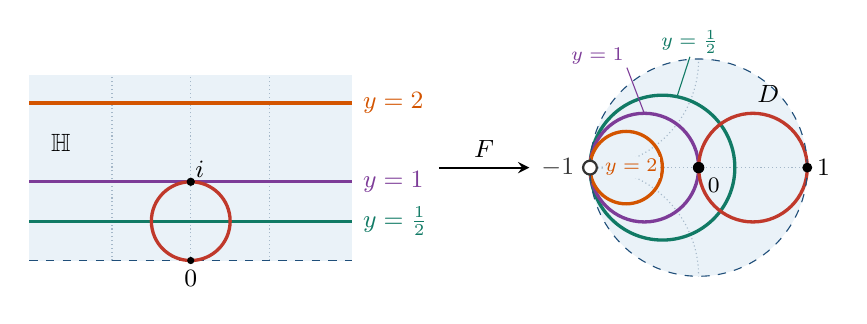
\begin{tikzpicture}[>=stealth,font=\small]
 % Left: horocycles (horospheres) in H
 \begin{scope}[scale=1.0]
  \fill[lightblue] (-2.05,0) rectangle (2.05,2.35);
  \draw[courseblue!40,densely dotted] (-1,0) -- (-1,2.35);
  \draw[courseblue!40,densely dotted] (0,0) -- (0,2.35);
  \draw[courseblue!40,densely dotted] (1,0) -- (1,2.35);
  \draw[courseblue,dashed] (-2.05,0) -- (2.05,0);
  % Horizontal lines (horocycles based at infinity)
  \draw[cayleyorange,very thick] (-2.05,2) -- (2.05,2) node[right,text=cayleyorange] {$y=2$};
  \draw[cayleypurple,very thick] (-2.05,1) -- (2.05,1) node[right,text=cayleypurple] {$y=1$};
  \draw[cayleyteal,very thick] (-2.05,0.5) -- (2.05,0.5) node[right,text=cayleyteal] {$y=\frac12$};
  % Finite-base horocycle tangent to R at 0
  \draw[cayleyred,very thick] (0,0.5) circle (0.5);
  \fill (0,0) circle (1.3pt) node[below] {$0$};
  \fill (0,1) circle (1.5pt) node[above right,inner sep=1.5pt] {$i$};
  \node at (-1.65,1.5) {$\mathbb H$};
 \end{scope}

 % Mapping arrow
 \draw[->,thick] (3.15,1.18) -- node[above] {$F$} (4.3,1.18);

 % Right: horocycles in D
 \begin{scope}[shift={(6.45,1.18)},scale=1.38]
  \fill[lightblue] (0,0) circle (1);
  \begin{scope}
   \clip (0,0) circle (1);
   \draw[courseblue!40,densely dotted] (-1,0) -- (1,0);
   \draw[courseblue!40,densely dotted] (-1,0) arc[start angle=-90,end angle=0,radius=1];
   \draw[courseblue!40,densely dotted] (-1,0) arc[start angle=90,end angle=0,radius=1];
  \end{scope}
  % Images of horizontal lines: circles internally tangent at -1
  \draw[cayleyteal,very thick] (-1/3,0) circle (2/3);
  \draw[cayleypurple,very thick] (-1/2,0) circle (1/2);
  \draw[cayleyorange,very thick] (-2/3,0) circle (1/3);
  % Image of horocycle at 0: circle internally tangent at +1
  \draw[cayleyred,very thick] (1/2,0) circle (1/2);
  \draw[courseblue,dashed] (0,0) circle (1);
  \fill (1,0) circle (1.3pt) node[right] {$1$};
  \fill (0,0) circle (1.5pt);
  \node[font=\footnotesize] at (0.14,-0.16) {$0$};
  \draw[darkgray,thick,fill=white] (-1,0) circle (1.8pt) node[left,xshift=-2pt] {$-1$};
  % Clean non-overlapping labels with external pins for top horocycles
  \node[text=cayleyorange,font=\scriptsize,fill=lightblue,inner sep=0.8pt] at (-0.62,0.0) {$y=2$};
  \draw[cayleypurple,thin] (-0.50,0.50) -- (-0.66,0.92) node[above left,inner sep=1pt,text=cayleypurple,font=\scriptsize] {$y=1$};
  \draw[cayleyteal,thin] (-0.20,0.65) -- (-0.08,1.02) node[above,inner sep=1pt,text=cayleyteal,font=\scriptsize] {$y=\frac12$};
  \node at (0.64,0.68) {$D$};
 \end{scope}
\end{tikzpicture}

\vspace{0.2em}
{\small\textbf{Horocycles (horospheres):} Horizontal lines $\Imag z=c>0$
(horocycles based at $\infty$) map to circles in $D$ internally tangent to
$\partial D$ at $-1$, with center $(-\frac{c}{1+c},0)$ and radius
$\frac{1}{1+c}$, orthogonal to the vertical geodesics (dotted). A circle
in $\mathbb H$ tangent to $\R$ at $0$ (red, horocycle based at $0$) maps to
a circle internally tangent to $\partial D$ at $1=F(0)$.}
\end{minipage}
\end{lecturefigure}


\subsection{Outside and inside the semicircle}

\begin{example}[The map $z+1/z$]
Set $U=\{z\in\mathbb H:|z|>1\}$ and let $J(z)=z+1/z$.
Writing $z=x+iy$ gives
\[
 J(z)=x(1+|z|^{-2})+iy(1-|z|^{-2}).
\]
Thus $J(U)\subseteq\mathbb H$. 

Suppose $J(z)=w$, i.e. we have a solution for $w\in\mathbb H$ of the equation
$z^2-wz+1=0$; the roots have product $1$, and neither is on the unit circle, where
$J(e^{it})=2\cos t$ is real. So, exactly one root has $|z|>1$, and since \be{} \Im(z + 1/z) = y ( 1 - \frac{1}{x^2+y^2}), \ee this root will lie in $U$ (the other one will not be in $U$ of course as $|z|<1$). Thus $J:U\to\mathbb H$
is bijective. Since $J$ is holomorphic, the result on holomorphic inverses
from Lecture~27 shows that $J$ is an analytic isomorphism.
\end{example}

\begin{exercise}[Boundary values]
Show that the two real rays of $\partial U$ map to $(-\infty,-2]$
and $[2,\infty)$, respectively. Use $J(e^{it})=2\cos t$ to check the
image of the semicircle.

\begin{lecturefigure}
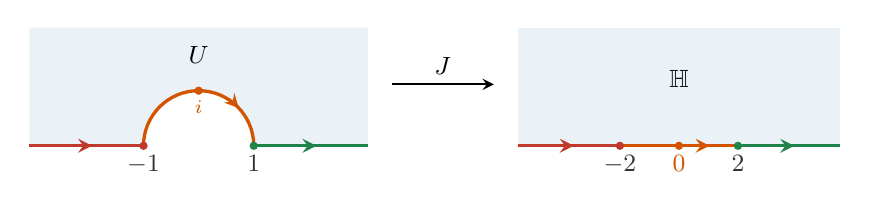
\begin{tikzpicture}[>=stealth,font=\small,
 midarrow/.style={postaction={decorate},decoration={markings,mark=at position .55 with {\arrow{>}}}},
 arcarrow/.style={postaction={decorate},decoration={markings,mark=at position .76 with {\arrow{>}}}}]
 % Left: U = {z in H : |z| > 1}
 \fill[lightblue] (-2.15,0) -- (-0.7,0) arc (180:0:0.7) -- (2.15,0)
  -- (2.15,1.5) -- (-2.15,1.5) -- cycle;
 \draw[cayleyred,very thick,midarrow] (-2.15,0) -- (-0.7,0);
 \draw[cayleyorange,very thick,arcarrow] (-0.7,0) arc (180:0:0.7);
 \draw[cayleygreen,very thick,midarrow] (0.7,0) -- (2.15,0);
 \fill[cayleyred] (-0.7,0) circle (1.5pt) node[below,text=darkgray] {$-1$};
 \fill[cayleyorange] (0,0.7) circle (1.5pt) node[below,font=\scriptsize,text=cayleyorange] {$i$};
 \fill[cayleygreen] (0.7,0) circle (1.5pt) node[below,text=darkgray] {$1$};
 \node at (0,1.15) {$U$};
 % Arrow
 \draw[->,thick] (2.45,0.78) -- node[above] {$J$} (3.75,0.78);
 % Right: H
 \fill[lightblue] (4.05,0) rectangle (8.15,1.5);
 \draw[cayleyred,very thick,midarrow] (4.05,0) -- (5.35,0);
 \draw[cayleyorange,very thick,arcarrow] (5.35,0) -- (6.85,0);
 \draw[cayleygreen,very thick,midarrow] (6.85,0) -- (8.15,0);
 \fill[cayleyred] (5.35,0) circle (1.5pt) node[below,text=darkgray] {$-2$};
 \fill[cayleyorange] (6.1,0) circle (1.5pt) node[below,text=cayleyorange] {$0$};
 \fill[cayleygreen] (6.85,0) circle (1.5pt) node[below,text=darkgray] {$2$};
 \node at (6.1,0.85) {$\mathbb H$};
\end{tikzpicture}

\vspace{0.15em}
{\small Under $J$, $(-\infty,-1]$ (red) maps to $(-\infty,-2]$, the
semicircle (orange, with $i\mapsto 0$) maps to $[-2,2]$, and
$[1,\infty)$ (green) maps to $[2,\infty)$.}
\end{lecturefigure}
\end{exercise}

\begin{example}[The open upper half-disc]\label{ex:upper-half-disc}
For $z\in\mathbb H$ with $|z|<1$, the point $-1/z$ belongs to $U$.
In fact $z\mapsto-1/z$ is an involution and exchanges these two regions.
Thus $\Phi(z)=-\tfrac12(z+1/z)=\tfrac12J(-1/z)$ maps the open upper
half-disc $D_+=\{z\in\mathbb H:|z|<1\}$ isomorphically onto $\mathbb H$.

\begin{lecturefigure}
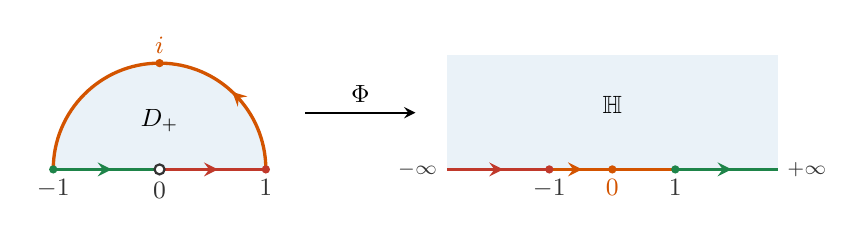
\begin{tikzpicture}[>=stealth,font=\small,
 midarrow/.style={postaction={decorate},decoration={markings,mark=at position .55 with {\arrow{>}}}},
 arcarrow/.style={postaction={decorate},decoration={markings,mark=at position .26 with {\arrow{>}}}}]
 % Left: D_+ = {z in H : |z| < 1}
 \fill[lightblue] (-1.35,0) -- (1.35,0) arc (0:180:1.35) -- cycle;
 \draw[cayleygreen,very thick,midarrow] (-1.35,0) -- (0,0);
 \draw[cayleyred,very thick,midarrow] (0,0) -- (1.35,0);
 \draw[cayleyorange,very thick,arcarrow] (1.35,0) arc (0:180:1.35);
 \fill[cayleygreen] (-1.35,0) circle (1.5pt) node[below,text=darkgray] {$-1$};
 \draw[darkgray,thick,fill=white] (0,0) circle (1.8pt) node[below,yshift=-1pt,text=darkgray] {$0$};
 \fill[cayleyred] (1.35,0) circle (1.5pt) node[below,text=darkgray] {$1$};
 \fill[cayleyorange] (0,1.35) circle (1.5pt) node[above,text=cayleyorange] {$i$};
 \node at (0,0.62) {$D_+$};
 % Arrow
 \draw[->,thick] (1.85,0.72) -- node[above] {$\Phi$} (3.25,0.72);
 % Right: H
 \fill[lightblue] (3.65,0) rectangle (7.85,1.45);
 \draw[cayleyred,very thick,midarrow] (3.65,0) -- (4.95,0);
 \draw[cayleyorange,very thick,arcarrow] (4.95,0) -- (6.55,0);
 \draw[cayleygreen,very thick,midarrow] (6.55,0) -- (7.85,0);
 \fill[cayleyred] (4.95,0) circle (1.5pt) node[below,text=darkgray] {$-1$};
 \fill[cayleyorange] (5.75,0) circle (1.5pt) node[below,text=cayleyorange] {$0$};
 \fill[cayleygreen] (6.55,0) circle (1.5pt) node[below,text=darkgray] {$1$};
 \node[left,text=darkgray,font=\scriptsize] at (3.65,0) {$-\infty$};
 \node[right,text=darkgray,font=\scriptsize] at (7.85,0) {$+\infty$};
 \node at (5.75,0.82) {$\mathbb H$};
\end{tikzpicture}

\vspace{0.15em}
{\small Under $\Phi(z)=-\tfrac12(z+1/z)$, $(0,1]$ (red) maps to $(-\infty,-1]$,
the semicircle from $1$ through $i$ to $-1$ (orange, with $i\mapsto 0$) maps to
$[-1,1]$, and $[-1,0)$ (green) maps to $[1,\infty)$, with $0\to\pm\infty$.}
\end{lecturefigure}
\end{example}

\subsection{Sectors and strips}

\begin{example}[A sector]
For a positive integer $n$, the map $z\mapsto z^n$ takes the sector
$\{re^{i\theta}:r>0,\ 0<\theta<\pi/n\}$ isomorphically onto
$\mathbb H$. It sends $re^{i\theta}$ to $r^ne^{in\theta}$.
Its inverse is $w\mapsto e^{(\log w)/n}$, with $0<\Arg w<\pi$ on
$\mathbb H$.
\end{example}

\begin{lecturefigure}
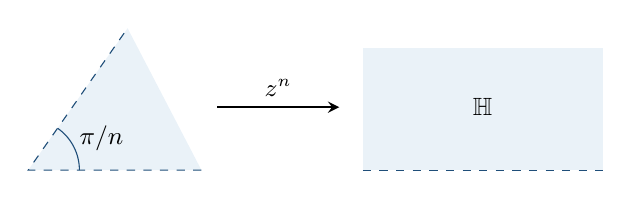
\begin{tikzpicture}[>=stealth,font=\small]
 \fill[lightblue] (0,0) -- (2.2,0) -- (55:2.2) -- cycle;
 \draw[courseblue,dashed] (2.2,0) -- (0,0) -- (55:2.2);
 \draw[courseblue] (0.65,0) arc (0:55:0.65);
 \node at (0.93,0.4) {$\pi/n$};
 \draw[->,thick] (2.4,0.8) -- node[above] {$z^n$} (3.95,0.8);
 \fill[lightblue] (4.25,0) rectangle (7.3,1.55);
 \draw[courseblue,dashed] (4.25,0) -- (7.3,0);
 \node at (5.77,0.8) {$\mathbb H$};
\end{tikzpicture}
\end{lecturefigure}

\begin{example}[Logarithm]
Take the branch $\log(re^{i\theta})=\log r+i\theta$ with
$-\pi/2<\theta<3\pi/2$, defined off the closed negative imaginary ray.
It maps $\mathbb H$ onto the strip $0<\Imag w<\pi$ and the open upper
half-disc onto the half-strip $\Real w<0$, $0<\Imag w<\pi$.
Both inverse maps are restrictions of $w\mapsto e^w$.

\begin{lecturefigure}
\begin{minipage}{\linewidth}\centering
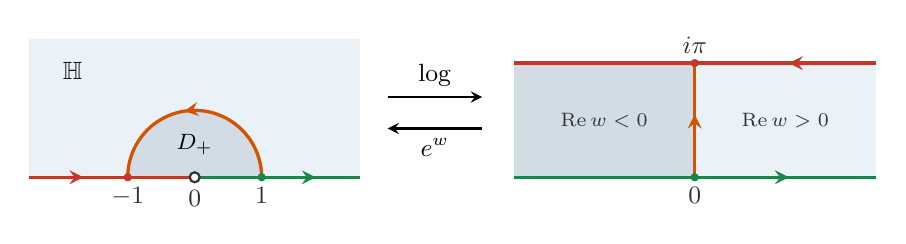
\begin{tikzpicture}[>=stealth,font=\small,
 midarrow/.style={postaction={decorate},decoration={markings,mark=at position .55 with {\arrow{>}}}}]
 % Left: H with D_+ shaded darker
 \fill[lightblue] (-2.1,0) rectangle (2.1,1.75);
 \fill[courseblue!20] (-0.85,0) -- (0.85,0) arc (0:180:0.85) -- cycle;
 \draw[cayleyred,very thick,midarrow] (-2.1,0) -- (-0.85,0);
 \draw[cayleyred,very thick] (-0.85,0) -- (0,0);
 \draw[cayleygreen,very thick] (0,0) -- (0.85,0);
 \draw[cayleygreen,very thick,midarrow] (0.85,0) -- (2.1,0);
 \draw[cayleyorange,very thick,midarrow] (0.85,0) arc (0:180:0.85);
 \fill[cayleyred] (-0.85,0) circle (1.5pt) node[below,text=darkgray] {$-1$};
 \fill[cayleygreen] (0.85,0) circle (1.5pt) node[below,text=darkgray] {$1$};
 \draw[darkgray,thick,fill=white] (0,0) circle (1.8pt) node[below,yshift=-1pt,text=darkgray] {$0$};
 \node[font=\footnotesize] at (0,0.42) {$D_+$};
 \node at (-1.55,1.35) {$\mathbb H$};

 % Arrows log / e^w
 \draw[->,thick] (2.45,1.02) -- node[above] {$\log$} (3.65,1.02);
 \draw[<-,thick] (2.45,0.62) -- node[below] {$e^w$} (3.65,0.62);

 % Right: strip 0 < Im w < pi (left half-strip shaded darker)
 \fill[courseblue!20] (4.05,0) rectangle (6.35,1.45);
 \fill[lightblue] (6.35,0) rectangle (8.65,1.45);
 \draw[cayleygreen,very thick,postaction={decorate},decoration={markings,mark=at position .76 with {\arrow{>}}}] (4.05,0) -- (8.65,0);
 \draw[cayleyred,very thick,postaction={decorate},decoration={markings,mark=at position .24 with {\arrow{>}}}] (8.65,1.45) -- (4.05,1.45);
 \draw[cayleyorange,very thick,midarrow] (6.35,0) -- (6.35,1.45);
 \fill[cayleygreen] (6.35,0) circle (1.5pt) node[below,text=darkgray] {$0$};
 \fill[cayleyred] (6.35,1.45) circle (1.5pt) node[above,text=darkgray] {$i\pi$};
 \node[font=\scriptsize,text=darkgray] at (5.2,0.72) {$\Real w<0$};
 \node[font=\scriptsize,text=darkgray] at (7.5,0.72) {$\Real w>0$};
\end{tikzpicture}

\vspace{0.15em}
{\small Under $\log$, $(0,\infty)$ (green) maps to $\Imag w=0$, $(-\infty,0)$
(red) maps to $\Imag w=\pi$, and the semicircle $|z|=1$ (orange) maps to the
vertical segment $[0,i\pi]$, separating the image of $D_+$ ($\Real w<0$) from
$\Real w>0$.}
\end{minipage}
\end{lecturefigure}
\end{example}
\begin{example}[Exponential]
On the vertical half-strip $|\Real z|<\pi/2$, $\Imag z>0$, the map
$z=x+iy\mapsto e^{iz}=e^{-y}e^{ix}$ sends it isomorphically to the open right
half-disc. Multiplication by $i$ then gives the upper half-disc, which
Example~\ref{ex:upper-half-disc} maps to $\mathbb H$.

\begin{lecturefigure}
\begin{minipage}{\linewidth}\centering
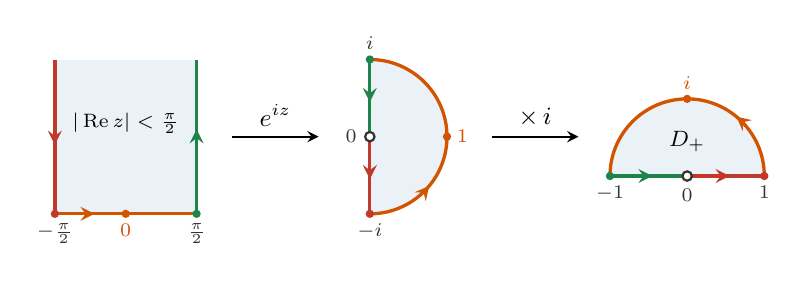
\begin{tikzpicture}[>=stealth,font=\small,
 midarrow/.style={postaction={decorate},decoration={markings,mark=at position .55 with {\arrow{>}}}},
 arcarrow/.style={postaction={decorate},decoration={markings,mark=at position .28 with {\arrow{>}}}}]
 % Left: vertical half-strip |Re z| < pi/2, Im z > 0
 \fill[lightblue] (-0.9,0) rectangle (0.9,1.95);
 \draw[cayleyred,very thick,midarrow] (-0.9,1.95) -- (-0.9,0);
 \draw[cayleyorange,very thick,arcarrow] (-0.9,0) -- (0.9,0);
 \draw[cayleygreen,very thick,midarrow] (0.9,0) -- (0.9,1.95);
 \fill[cayleyred] (-0.9,0) circle (1.5pt) node[below,font=\scriptsize,text=darkgray] {$-\frac{\pi}{2}$};
 \fill[cayleyorange] (0,0) circle (1.5pt) node[below,font=\scriptsize,text=cayleyorange] {$0$};
 \fill[cayleygreen] (0.9,0) circle (1.5pt) node[below,font=\scriptsize,text=darkgray] {$\frac{\pi}{2}$};
 \node[font=\scriptsize] at (0,1.15) {$|\Real z|<\frac{\pi}{2}$};

 % Arrow e^{iz}
 \draw[->,thick] (1.35,0.98) -- node[above] {$e^{iz}$} (2.45,0.98);

 % Middle: open right half-disc
 \fill[lightblue] (3.1,0) arc (-90:90:0.98) -- cycle;
 \draw[cayleyred,very thick,midarrow] (3.1,0.98) -- (3.1,0);
 \draw[cayleyorange,very thick,arcarrow] (3.1,0) arc (-90:90:0.98);
 \draw[cayleygreen,very thick,midarrow] (3.1,1.96) -- (3.1,0.98);
 \fill[cayleyred] (3.1,0) circle (1.5pt) node[below,font=\scriptsize,text=darkgray] {$-i$};
 \fill[cayleyorange] (4.08,0.98) circle (1.5pt) node[right,font=\scriptsize,text=cayleyorange] {$1$};
 \fill[cayleygreen] (3.1,1.96) circle (1.5pt) node[above,font=\scriptsize,text=darkgray] {$i$};
 \draw[darkgray,thick,fill=white] (3.1,0.98) circle (1.7pt) node[left,xshift=-1pt,font=\scriptsize,text=darkgray] {$0$};

 % Arrow x i
 \draw[->,thick] (4.65,0.98) -- node[above] {$\times\,i$} (5.75,0.98);

 % Right: open upper half-disc D_+
 \fill[lightblue] (6.15,0.48) -- (8.11,0.48) arc (0:180:0.98) -- cycle;
 \draw[cayleygreen,very thick,midarrow] (6.15,0.48) -- (7.13,0.48);
 \draw[cayleyred,very thick,midarrow] (7.13,0.48) -- (8.11,0.48);
 \draw[cayleyorange,very thick,arcarrow] (8.11,0.48) arc (0:180:0.98);
 \fill[cayleygreen] (6.15,0.48) circle (1.5pt) node[below,font=\scriptsize,text=darkgray] {$-1$};
 \fill[cayleyred] (8.11,0.48) circle (1.5pt) node[below,font=\scriptsize,text=darkgray] {$1$};
 \fill[cayleyorange] (7.13,1.46) circle (1.5pt) node[above,font=\scriptsize,text=cayleyorange] {$i$};
 \draw[darkgray,thick,fill=white] (7.13,0.48) circle (1.7pt) node[below,yshift=-1pt,font=\scriptsize,text=darkgray] {$0$};
 \node[font=\footnotesize] at (7.13,0.92) {$D_+$};
\end{tikzpicture}

\vspace{0.15em}
{\small Under $e^{iz}$ and then multiplication by $i$, the bottom edge
$[-\frac{\pi}{2},\frac{\pi}{2}]$ (orange, with $0\mapsto 1\mapsto i$) maps
to the semicircle, while the left (red) and right (green) vertical rays map
to the radii $(0,1]$ and $[-1,0)$, with $\Imag z\to+\infty$ sent to $0$.}
\end{minipage}
\end{lecturefigure}
\end{example}

% Source: handwritten Lecture 28, Nov. 25, pp. 1--7.
\section{The Fourier transform}

A Fourier transform describes a function $f$ of a real variable $x$ in terms of its `frequency'
 $\xi \in \R$. On the real line it is defined as
\[
 \widehat f(\xi)=\int_{-\infty}^{\infty} f(x)e^{-2\pi i x\xi}\,dx,
 \qquad \xi\in\R.
\]

Notice that the answer is a complex-valued function. Why does this integral exist? And what does it mean?

Let me come back to well-definedness in a moment, but let's look at the following pictures to get some intuition for it.

\begin{example}[A pure cosine wave: $f(x)=\cos(2\pi ax)$]
Fix a frequency $a>0$, and consider $f(x)=\cos(2\pi ax)$ and its Fourier transform:
\be{} \widehat f (\xi)  = \int_{- \infty}^{\infty} \cos(2\pi ax) e^{ - 2 \pi i x \xi } \,dx. \ee
The imaginary part of the integrand is $-\cos(2\pi ax) \sin(2 \pi \xi x)$, an odd function, so its integral over any interval centered at $0$ vanishes.Hence, in this case the Fourier transform (if it exists) should be equal to its real part. What should it look like ? Since
\[
 \cos(2\pi ax) = \frac{1}{2}e^{2\pi iax} + \frac{1}{2}e^{-2\pi iax},
\]
the expectation is that it should have two spikes at $\pm a$ and be zero elsewhere--- said another way, $\cos(2 \pi ax)$ is a superposition of two pure oscillations at frequencies
$\xi=\pm a$ (it has period $1/a$, completing $a$ cycles per unit $x$). In other words, we expect the picture of the Fourier transform to look like:

\begin{lecturefigure}
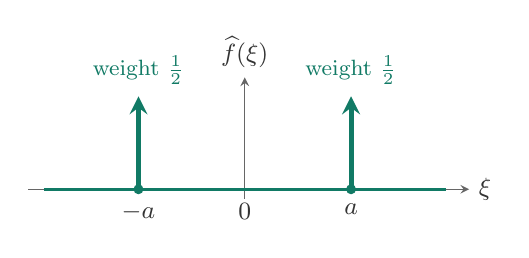
\begin{tikzpicture}[>=stealth,font=\small]
 % Axes
 \draw[->,darkgray!75] (-2.75,0) -- (2.85,0) node[right,text=darkgray] {$\xi$};
 \draw[->,darkgray!75] (0,-0.12) -- (0,1.42) node[above,text=darkgray] {$\widehat{f}(\xi)$};
 % Thick zero-baseline showing zero elsewhere
 \draw[cayleyteal,line width=1.2pt] (-2.55,0) -- (2.55,0);
 % Ticks at -a, 0, a
 \draw[darkgray!75] (-1.35,0.06) -- (-1.35,-0.06) node[below,text=darkgray] {$-a$};
 \draw[darkgray!75] (1.35,0.06) -- (1.35,-0.06) node[below,text=darkgray] {$a$};
 \node[below,text=darkgray] at (0,-0.06) {$0$};
 % Two idealized spikes at xi = +-a
 \draw[->,cayleyteal,line width=1.8pt] (-1.35,0) -- (-1.35,1.18)
  node[above,font=\footnotesize,text=cayleyteal] {weight $\tfrac{1}{2}$};
 \draw[->,cayleyteal,line width=1.8pt] (1.35,0) -- (1.35,1.18)
  node[above,font=\footnotesize,text=cayleyteal] {weight $\tfrac{1}{2}$};
 \fill[cayleyteal] (-1.35,0) circle (1.8pt);
 \fill[cayleyteal] (1.35,0) circle (1.8pt);
\end{tikzpicture}
\end{lecturefigure}



In reality, $\cos(2\pi ax)$ does not decay as
$|x|\to\infty$, so the improper integral
$\int_{-\infty}^{\infty}\cos(2\pi ax)e^{-2\pi ix\xi}\,dx$ does not
converge! There are workarounds though: consider the truncated integral
over $[-L,L]$:
\[
 I_L(\xi) = \int_{-L}^{L}\cos(2\pi ax)e^{-2\pi ix\xi}\,dx
          = \int_{-L}^{L}\cos(2\pi ax)\cos(2\pi\xi x)\,dx.
\]

Use the product-to-sum identity
\[
 \cos A\cos B = \tfrac12\bigl[\cos(A-B)+\cos(A+B)\bigr].
\]
With $A=2\pi ax$ and $B=2\pi\xi x$, we get, for $\xi\ne\pm a$,
\begin{align*}
 I_L(\xi)
  &= \frac12\int_{-L}^{L}
     \bigl[\cos(2\pi(a-\xi)x)+\cos(2\pi(a+\xi)x)\bigr]\,dx \\
  &= \frac12\left[
      \frac{\sin\bigl(2\pi(a-\xi)x\bigr)}{2\pi(a-\xi)}
    + \frac{\sin\bigl(2\pi(a+\xi)x\bigr)}{2\pi(a+\xi)}
     \right]_{-L}^{L} \\
  &= \frac{\sin\bigl(2\pi L(a-\xi)\bigr)}{2\pi(a-\xi)}
   + \frac{\sin\bigl(2\pi L(a+\xi)\bigr)}{2\pi(a+\xi)}.
\end{align*}
At $\xi=\pm a$, the term with zero denominator is replaced by $L$, since
the corresponding integrand is $\tfrac12\cos(0)=\tfrac12$ on $[-L,L]$. When $\xi\ne\pm a$, the integrand oscillates and cancels, keeping
$I_L(\xi)$ bounded as $L\to\infty$. The terms that grow at $\xi=\pm a$
give $I_L(\xi)$ two tall, narrow
peaks centered at $\xi=\pm a$, each enclosing total area $\frac{1}{2}$
(using $\int_{-\infty}^{\infty}\frac{\sin u}{u}\,du=\pi$). In the limit
$L\to\infty$, the Fourier transform of $\cos(2\pi ax)$ is concentrated
into two idealized spikes (Dirac impulses) of weight $\frac{1}{2}$ at
$\xi=\pm a$, written formally as
\[
 \widehat{f}(\xi)
  = \frac{1}{2}\delta(\xi-a) + \frac{1}{2}\delta(\xi+a).
\]
with $\delta(x)$ being the Dirac delta function, i.e. equal to $1$ at $x=0$ and being equal to $0$ elsewhere.

\begin{lecturefigure}
\begin{minipage}{\linewidth}\centering
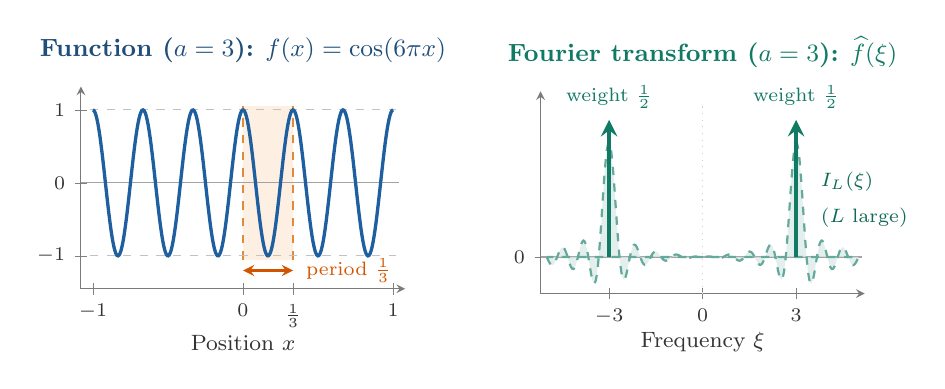
\begin{tikzpicture}[>=stealth]
 % Left panel: f(x) = cos(6 pi x)  (a = 3)
 \begin{axis}[
   name=leftplot,
   width=0.47\linewidth,
   height=4.15cm,
   axis lines=left,
   axis line style={darkgray!65},
   xmin=-1.08, xmax=1.08,
   ymin=-1.45, ymax=1.32,
   xtick={-1, 0, 0.333333, 1},
   xticklabels={$-1$, $0$, $\frac{1}{3}$, $1$},
   ytick={-1, 0, 1},
   yticklabels={$-1$, $0$, $1$},
   tick label style={font=\scriptsize, text=darkgray},
   xlabel={Position $x$},
   xlabel style={font=\footnotesize, text=darkgray, yshift=4pt},
   title={\textbf{Function ($a=3$):} $f(x)=\cos(6\pi x)$},
   title style={font=\small, text=courseblue, yshift=-1pt},
   clip=false
  ]
  % Highlight one full period [0, 1/3]
  \fill[lightorange, fill opacity=0.75] (axis cs:0,-1.05) rectangle (axis cs:0.333333,1.05);
  \draw[orangeframe, dashed, thin] (axis cs:0,-1.05) -- (axis cs:0,1.05);
  \draw[orangeframe, dashed, thin] (axis cs:0.333333,-1.05) -- (axis cs:0.333333,1.05);
  % Reference baselines y = 0, +-1
  \draw[darkgray!45, thin] (axis cs:-1.08,0) -- (axis cs:1.04,0);
  \draw[darkgray!30, dashed, thin] (axis cs:-1.02,1) -- (axis cs:1.02,1);
  \draw[darkgray!30, dashed, thin] (axis cs:-1.02,-1) -- (axis cs:1.02,-1);
  % Plot cos(6 pi x)
  \addplot[cayleyblue, very thick, domain=-1:1, samples=300] {cos(1080*x)};
  % Period callout to the right of the [0, 1/3] arrow
  \draw[<->, cayleyorange, thick] (axis cs:0,-1.20) -- (axis cs:0.333333,-1.20)
   node[right, xshift=1pt, font=\scriptsize, text=cayleyorange] {period $\frac{1}{3}$};
 \end{axis}

 % Right panel: Fourier transform of cos(6 pi x)  (a = 3)
 \begin{axis}[
   at={(leftplot.outer east)}, anchor=outer west, xshift=0.55cm,
   width=0.47\linewidth,
   height=4.15cm,
   axis lines=left,
   axis line style={darkgray!65},
   xmin=-5.2, xmax=5.2,
   ymin=-0.32, ymax=1.45,
   xtick={-3, 0, 3},
   xticklabels={$-3$, $0$, $3$},
   ytick={0},
   yticklabels={$0$},
   tick label style={font=\scriptsize, text=darkgray},
   xlabel={Frequency $\xi$},
   xlabel style={font=\footnotesize, text=darkgray, yshift=4pt},
   title={\textbf{Fourier transform ($a=3$):} $\widehat{f}(\xi)$},
   title style={font=\small, text=cayleyteal, yshift=-1pt},
   clip=false
  ]
  % Reference baseline y = 0 and center line xi = 0
  \draw[darkgray!45, thin] (axis cs:-5.2,0) -- (axis cs:5.1,0);
  \draw[darkgray!25, dotted, thin] (axis cs:0,-0.32) -- (axis cs:0,1.35);
  % Truncated integral I_L(xi)/L for L = 1.5 (shows narrowing peaks at +-3)
  \addplot[
    cayleyteal!65, dashed, thick,
    fill=cayleyteal!15, fill opacity=0.8,
    domain=-5.0:5.0, samples=281
  ] {
    (abs(3 - x) < 0.0001 ? 1 : sin(540*(3 - x))/(9.424778*(3 - x)))
    +
    (abs(3 + x) < 0.0001 ? 1 : sin(540*(3 + x))/(9.424778*(3 + x)))
  } \closedcycle;
  % Limiting Dirac impulses at xi = +-3
  \draw[->, cayleyteal, line width=1.6pt] (axis cs:-3,0) -- (axis cs:-3,1.20)
   node[above, font=\scriptsize, text=cayleyteal] {weight $\frac{1}{2}$};
  \draw[->, cayleyteal, line width=1.6pt] (axis cs:3,0) -- (axis cs:3,1.20)
   node[above, font=\scriptsize, text=cayleyteal] {weight $\frac{1}{2}$};
  % Annotation for the dashed finite-window curve
  \node[font=\scriptsize, text=cayleyteal!85!black, anchor=west] at (axis cs:3.48,0.66) {$I_L(\xi)$};
  \node[font=\scriptsize, text=cayleyteal!85!black, anchor=west] at (axis cs:3.48,0.34) {($L$ large)};
 \end{axis}
\end{tikzpicture}

\vspace{0.1em}
{\small\textbf{Pure cosine wave ($a=3$):} $f(x)=\cos(6\pi x)$ completes
$3$ full periods per unit $x$ (period $\frac{1}{3}$). The truncated
integral $I_L(\xi)$ (dashed, scaled) peaks sharply at $\xi=\pm 3$ and
concentrates as $L\to\infty$ into two spikes of weight $\frac{1}{2}$ at
$\xi=\pm 3$.}
\end{minipage}
\end{lecturefigure}
\end{example}

\begin{example}[A pure sine wave: $f(x)=\sin(2\pi ax)$]
For $a>0$, now consider $f(x)=\sin(2\pi ax)$ and its Fourier transform:
\[
 \widehat f(\xi) = \int_{-\infty}^{\infty}\sin(2\pi ax)e^{-2\pi ix\xi}\,dx
  = \int_{-\infty}^{\infty}\sin(2\pi ax)\cos(2\pi\xi x)\,dx
  - i\int_{-\infty}^{\infty}\sin(2\pi ax)\sin(2\pi\xi x)\,dx.
\]
This time the \emph{real} part of the integrand, $\sin(2\pi ax)\cos(2\pi\xi x)$,
is an odd function of $x$, so its integral over any interval centered at
$0$ vanishes. Hence we focus on the \emph{imaginary} part of $\widehat f(\xi)$:
its integrand $-\sin(2\pi ax)\sin(2\pi\xi x)$ is even, and at $\xi=a$ it
equals $-\sin^2(2\pi ax)\le 0$ while at $\xi=-a$ it equals
$+\sin^2(2\pi ax)\ge 0$.

By Euler's formula, $\sin(2\pi ax)$ is a \emph{difference} of the two pure
exponentials $e^{\pm 2\pi iax}$ divided by $2i$:
\[
 \sin(2\pi ax) = \frac{e^{2\pi iax} - e^{-2\pi iax}}{2i}
               = -\frac{i}{2}e^{2\pi iax} + \frac{i}{2}e^{-2\pi iax}.
\]
Just as for $\cos(2\pi ax)$, the two exponentials $e^{2\pi iax}$ and
$e^{-2\pi iax}$ produce idealized spikes (Dirac impulses) at $\xi=a$ and
$\xi=-a$ respectively, and zero elsewhere. Because $\sin(2\pi ax)$ is their
\emph{difference} divided by $2i$, the coefficients $-\frac{i}{2}$ and
$+\frac{i}{2}$ are purely imaginary and have \emph{opposite signs}:
\[
 \widehat f(\xi)
  = \frac{1}{2i}\bigl(\delta(\xi-a)-\delta(\xi+a)\bigr)
  = i\Bigl(\frac{1}{2}\delta(\xi+a)-\frac{1}{2}\delta(\xi-a)\Bigr).
\]
Thus $\Imag\widehat f(\xi)$ has an upward spike of weight $+\frac{1}{2}$
at $\xi=-a$ and a downward spike of weight $-\frac{1}{2}$ at $\xi=a$.

\begin{lecturefigure}
\begin{minipage}{\linewidth}\centering
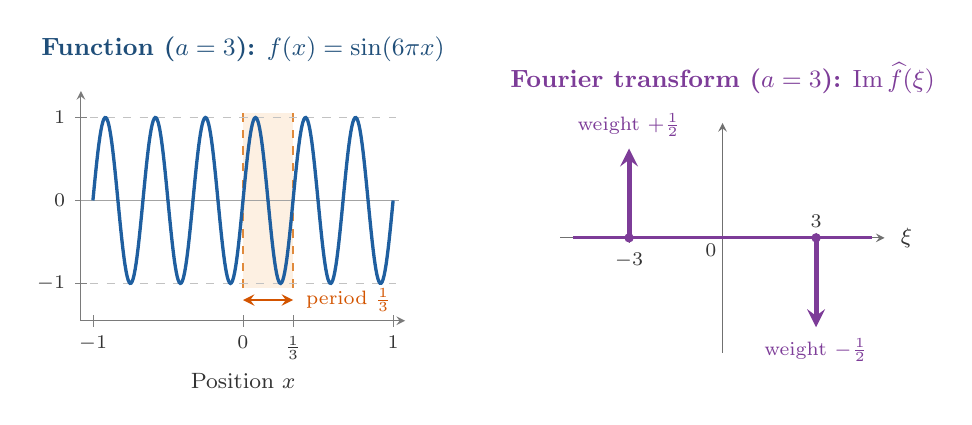
\begin{tikzpicture}[>=stealth]
 % Left panel: f(x) = sin(6 pi x)  (a = 3)
 \begin{axis}[
   name=sinleft,
   width=0.47\linewidth,
   height=4.5cm,
   axis lines=left,
   axis line style={darkgray!65},
   xmin=-1.08, xmax=1.08,
   ymin=-1.45, ymax=1.32,
   xtick={-1, 0, 0.333333, 1},
   xticklabels={$-1$, $0$, $\frac{1}{3}$, $1$},
   ytick={-1, 0, 1},
   yticklabels={$-1$, $0$, $1$},
   tick label style={font=\scriptsize, text=darkgray},
   xlabel={Position $x$},
   xlabel style={font=\footnotesize, text=darkgray, yshift=2pt},
   title={\textbf{Function ($a=3$):} $f(x)=\sin(6\pi x)$},
   title style={font=\small, text=courseblue, yshift=1pt},
   clip=false
  ]
  % Highlight one full period [0, 1/3]
  \fill[lightorange, fill opacity=0.75] (axis cs:0,-1.05) rectangle (axis cs:0.333333,1.05);
  \draw[orangeframe, dashed, thin] (axis cs:0,-1.05) -- (axis cs:0,1.05);
  \draw[orangeframe, dashed, thin] (axis cs:0.333333,-1.05) -- (axis cs:0.333333,1.05);
  % Reference baselines y = 0, +-1
  \draw[darkgray!45, thin] (axis cs:-1.08,0) -- (axis cs:1.04,0);
  \draw[darkgray!30, dashed, thin] (axis cs:-1.02,1) -- (axis cs:1.02,1);
  \draw[darkgray!30, dashed, thin] (axis cs:-1.02,-1) -- (axis cs:1.02,-1);
  % Plot sin(6 pi x)
  \addplot[cayleyblue, very thick, domain=-1:1, samples=300] {sin(1080*x)};
  % Period callout
  \draw[<->, cayleyorange, thick] (axis cs:0,-1.20) -- (axis cs:0.333333,-1.20)
   node[right, xshift=1pt, font=\scriptsize, text=cayleyorange] {period $\frac{1}{3}$};
 \end{axis}

 % Right panel: distributional Im f-hat(xi) for a = 3
 \begin{axis}[
   at={(sinleft.outer east)}, anchor=outer west, xshift=0.6cm,
   width=0.47\linewidth,
   height=4.5cm,
   axis lines=middle,
   axis line style={darkgray!70},
   xmin=-5.2, xmax=5.2,
   ymin=-1.35, ymax=1.35,
   xtick=\empty,
   ytick=\empty,
   xlabel={$\xi$},
   xlabel style={at={(axis description cs:1.02,0.5)}, anchor=west, font=\footnotesize, text=darkgray},
   title={\textbf{Fourier transform ($a=3$):} $\Imag\widehat f(\xi)$},
   title style={font=\small, text=cayleypurple, yshift=1pt},
   clip=false
  ]
  % Zero baseline showing zero elsewhere
  \draw[cayleypurple, line width=1.1pt] (axis cs:-4.8,0) -- (axis cs:4.8,0);
  % Ticks placed on opposite sides of the spikes to avoid any collision
  \draw[darkgray!70] (axis cs:-3,0.06) -- (axis cs:-3,-0.06) node[below, font=\scriptsize, text=darkgray] {$-3$};
  \draw[darkgray!70] (axis cs:3,0.06) -- (axis cs:3,-0.06) node[above, font=\scriptsize, text=darkgray, yshift=2pt] {$3$};
  \node[below left, font=\scriptsize, text=darkgray, inner sep=2pt] at (axis cs:0,0) {$0$};
  % Upward spike at xi = -3 (weight +1/2)
  \draw[->, cayleypurple, line width=1.8pt] (axis cs:-3,0) -- (axis cs:-3,1.05)
   node[above, font=\scriptsize, text=cayleypurple] {weight $+\frac{1}{2}$};
  \fill[cayleypurple] (axis cs:-3,0) circle (1.7pt);
  % Downward spike at xi = +3 (weight -1/2)
  \draw[->, cayleypurple, line width=1.8pt] (axis cs:3,0) -- (axis cs:3,-1.05)
   node[below, font=\scriptsize, text=cayleypurple] {weight $-\frac{1}{2}$};
  \fill[cayleypurple] (axis cs:3,0) circle (1.7pt);
 \end{axis}
\end{tikzpicture}

\vspace{0.2em}
{\small\textbf{Pure sine wave ($a=3$):} $f(x)=\sin(6\pi x)$ is odd, so
its distributional Fourier transform is purely imaginary, with
opposite-sign spikes of weight $+\frac{1}{2}$ at $\xi=-3$ and
$-\frac{1}{2}$ at $\xi=3$.}
\end{minipage}
\end{lecturefigure}
\end{example}

\begin{remark}[Differentiation and the Fourier transform]
For a smooth function $f$ decaying rapidly at $\pm\infty$, integration by
parts gives
\[
 \widehat{f'}(\xi)
  = \int_{-\infty}^{\infty} f'(x)e^{-2\pi ix\xi}\,dx
  = -\int_{-\infty}^{\infty} f(x)(-2\pi i\xi)e^{-2\pi ix\xi}\,dx
  = 2\pi i\xi\,\widehat{f}(\xi).
\]
That is, differentiation on the $x$-side becomes multiplication by
$2\pi i\xi$ on the frequency side. Formally, the same rule links the
preceding two examples: for $f(x)=\cos(2\pi ax)$ we have
$f'(x)=-2\pi a\sin(2\pi ax)$, and multiplying
$\widehat f(\xi)=\frac{1}{2}\delta(\xi-a)+\frac{1}{2}\delta(\xi+a)$ by
$2\pi i\xi$ (using $\xi\,\delta(\xi\mp a)=\pm a\,\delta(\xi\mp a)$) gives
\[
 \widehat{f'}(\xi)
  = 2\pi i\xi\Bigl(\frac{1}{2}\delta(\xi-a)+\frac{1}{2}\delta(\xi+a)\Bigr)
  = 2\pi ia\Bigl(\frac{1}{2}\delta(\xi-a)-\frac{1}{2}\delta(\xi+a)\Bigr).
\]
Dividing both sides by $-2\pi a$ recovers the Fourier transform of
$g(x)=\sin(2\pi ax)$,
\[
 \widehat{g}(\xi)
  = i\Bigl(\frac{1}{2}\delta(\xi+a)-\frac{1}{2}\delta(\xi-a)\Bigr).
\]
Geometrically, the factor $i$ rotates the purely real spikes of
$\cos(2\pi ax)$ into purely imaginary ones, while the factor $\xi$
multiplies the spike at $+a$ by $+a$ and the spike at $-a$ by $-a$,
giving them opposite signs.
\end{remark}

\begin{example}[The Gaussian: $g(x)=e^{-\pi x^2}$]
Unlike $\cos(2\pi ax)$ and $\sin(2\pi ax)$, the Gaussian $g(x)=e^{-\pi x^2}$
decays rapidly as $|x|\to\infty$, so its Fourier integral converges
absolutely for every $\xi\in\R$ and defines an honest smooth function.
In fact, we already computed this integral earlier in the course: in
Lecture~14 (Section~2, Theorem~2.1), using Cauchy's theorem to shift a
rectangular contour together with $\int_{-\infty}^{\infty}e^{-\pi x^2}\,dx=1$,
we proved that
\[
 \widehat g(\xi)
  = \int_{-\infty}^{\infty} e^{-\pi x^2}e^{-2\pi ix\xi}\,dx
  = e^{-\pi\xi^2} \qquad (\xi\in\R).
\]
Thus $e^{-\pi x^2}$ is \emph{its own Fourier transform}. More generally,
for any $\lambda>0$, setting $g_\lambda(x)=e^{-\pi\lambda x^2}$ and
substituting $u=\sqrt{\lambda}\,x$ gives
\[
 \widehat{g_\lambda}(\xi)
  = \frac{1}{\sqrt{\lambda}}
    \int_{-\infty}^{\infty} e^{-\pi u^2}e^{-2\pi iu(\xi/\sqrt{\lambda})}\,du
  = \frac{1}{\sqrt{\lambda}}\,e^{-\pi\xi^2/\lambda}.
\]
In particular, concentrating the Gaussian in position (taking $\lambda>1$
so $g_\lambda$ is narrower) spreads out its Fourier transform in
frequency, and vice versa.

\begin{lecturefigure}
\begin{minipage}{\linewidth}\centering
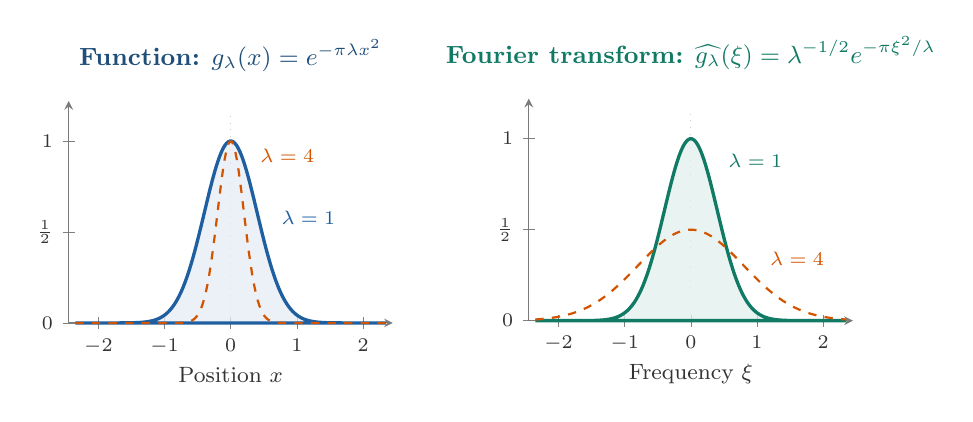
\begin{tikzpicture}[>=stealth]
 % Left panel: Gaussians in position x
 \begin{axis}[
   name=gaussleft,
   width=0.47\linewidth,
   height=4.4cm,
   axis lines=left,
   axis line style={darkgray!65},
   xmin=-2.45, xmax=2.45,
   ymin=0, ymax=1.22,
   xtick={-2, -1, 0, 1, 2},
   ytick={0, 0.5, 1},
   yticklabels={$0$, $\frac{1}{2}$, $1$},
   tick label style={font=\scriptsize, text=darkgray},
   xlabel={Position $x$},
   xlabel style={font=\footnotesize, text=darkgray, yshift=2pt},
   title={\textbf{Function:} $g_\lambda(x)=e^{-\pi\lambda x^2}$},
   title style={font=\small, text=courseblue, yshift=1pt},
   clip=false
  ]
  \draw[darkgray!25, dotted, thin] (axis cs:0,0) -- (axis cs:0,1.15);
  % lambda = 1
  \addplot[
    cayleyblue, very thick,
    fill=cayleyblue!12, fill opacity=0.75,
    domain=-2.35:2.35, samples=180
  ] {exp(-3.1415927*x*x)} \closedcycle;
  % lambda = 4 (narrower)
  \addplot[
    cayleyorange, dashed, thick,
    domain=-2.35:2.35, samples=180
  ] {exp(-4*3.1415927*x*x)};
  \node[font=\scriptsize, text=cayleyblue, anchor=west] at (axis cs:0.62,0.58) {$\lambda=1$};
  \node[font=\scriptsize, text=cayleyorange, anchor=west] at (axis cs:0.30,0.92) {$\lambda=4$};
 \end{axis}

 % Right panel: Fourier transforms in frequency xi
 \begin{axis}[
   at={(gaussleft.outer east)}, anchor=outer west, xshift=0.55cm,
   width=0.47\linewidth,
   height=4.4cm,
   axis lines=left,
   axis line style={darkgray!65},
   xmin=-2.45, xmax=2.45,
   ymin=0, ymax=1.22,
   xtick={-2, -1, 0, 1, 2},
   ytick={0, 0.5, 1},
   yticklabels={$0$, $\frac{1}{2}$, $1$},
   tick label style={font=\scriptsize, text=darkgray},
   xlabel={Frequency $\xi$},
   xlabel style={font=\footnotesize, text=darkgray, yshift=2pt},
   title={\textbf{Fourier transform:} $\widehat{g_\lambda}(\xi)=\lambda^{-1/2}e^{-\pi\xi^2/\lambda}$},
   title style={font=\small, text=cayleyteal, yshift=1pt},
   clip=false
  ]
  \draw[darkgray!25, dotted, thin] (axis cs:0,0) -- (axis cs:0,1.15);
  % lambda = 1
  \addplot[
    cayleyteal, very thick,
    fill=cayleyteal!12, fill opacity=0.75,
    domain=-2.35:2.35, samples=180
  ] {exp(-3.1415927*x*x)} \closedcycle;
  % lambda = 4 (wider)
  \addplot[
    cayleyorange, dashed, thick,
    domain=-2.35:2.35, samples=180
  ] {0.5*exp(-3.1415927*x*x/4)};
  \node[font=\scriptsize, text=cayleyteal, anchor=west] at (axis cs:0.42,0.88) {$\lambda=1$};
  \node[font=\scriptsize, text=cayleyorange, anchor=west] at (axis cs:1.05,0.34) {$\lambda=4$};
 \end{axis}
\end{tikzpicture}

\vspace{0.2em}
{\small\textbf{Gaussian and scaling:} For $\lambda=1$ (solid),
$e^{-\pi x^2}$ is fixed by the Fourier transform. For $\lambda=4$
(dashed), a narrower Gaussian in $x$ transforms into a wider Gaussian in
$\xi$.}
\end{minipage}
\end{lecturefigure}
\end{example}




\subsection{A convergence class}


Suppose that $f:\R\to\C$ is continuous and $|f(x)|\leq A/(1+x^2)$ for
some $A>0$ (we say $f$ is of \emph{moderate decay} if this holds). Then
we claim the Fourier integral defining $\widehat f(\xi)$ exists and in
fact \be{} |\widehat f(\xi)|\leq\pi A. \ee

\begin{proof}
Since $f$ is continuous, it is integrable on each bounded
interval. For real $x$ and $\xi$ we have $|e^{-2\pi i x\xi}|=1$, hence
\[
 \bigl|f(x)e^{-2\pi i x\xi}\bigr|=|f(x)|\leq\frac{A}{1+x^2}.
\]
The right-hand side is integrable on $\R$:
\[
 \int_{-\infty}^{\infty}\frac{dx}{1+x^2}
 =\lim_{R\to\infty}\bigl[\arctan x\bigr]_{-R}^{R}
 =\frac{\pi}{2}-\Bigl(-\frac{\pi}{2}\Bigr)=\pi .
\]
By the comparison test, the integral defining $\widehat f(\xi)$
converges absolutely, so $\widehat f(\xi)$ exists for every $\xi\in\R$.
Moving the absolute value inside the integral then gives
\[
 |\widehat f(\xi)|\leq\int_{-\infty}^{\infty}|f(x)|\,dx
 \leq A\int_{-\infty}^{\infty}\frac{dx}{1+x^2}=\pi A .
\]
The bound does not depend on $\xi$, so $\widehat f$ is bounded on $\R$.
\end{proof}


More generally, we consider the following class of functions.

\begin{definition}[Moderate decay on a strip]
For $a>0$ let $S_a=\{z\in\C:|\Imag z|<a\}$. Let $\mathcal F_a$ be
the class of holomorphic functions on $S_a$ for which there is a single
constant $A>0$ satisfying
\[
 |f(x+iy)|\leq\frac{A}{1+x^2}\qquad(x\in\R,\ |y|<a).
\]
We write $\mathcal F=\bigcup_{a>0}\mathcal F_a$, viewing these
functions on the real line with their holomorphic extensions to strips.
\end{definition}

\begin{example}[A Gaussian and a rational function]\mbox{}
\begin{itemize}
\item For $\lambda>0$, $e^{-\pi\lambda z^2}$ belongs to $\mathcal F_a$ for
every $a>0$, since its modulus is at most
$e^{\pi\lambda a^2}e^{-\pi\lambda x^2}$.

\item For $c>0$, the function $c/(c^2+z^2)$ belongs to $\mathcal F_a$ for
$0<a<c$. Its poles are at $\pm ic$, and for $|y|<a$,
$|c^2+(x+iy)^2|\geq c^2-a^2+x^2$. 
\end{itemize}
\end{example}


\section{Contour shifting and exponential decay}

\begin{theorem}[Shifting the Fourier integral]\label{thm:shift}
Let $f\in\mathcal F_a$ with constant $A$. For $|y|<a$ and $\xi\in\R$,
\begin{equation}\label{eq:shift}
 \widehat f(\xi)=\int_{-\infty}^{\infty}
 f(x+iy)e^{-2\pi i(x+iy)\xi}\,dx .
\end{equation}
In particular, for $0\leq b<a$,
\[
 |\widehat f(\xi)|\leq\pi A e^{-2\pi b|\xi|}.
\]
\end{theorem}

\begin{lecturefigure}
\begin{minipage}{\linewidth}\centering
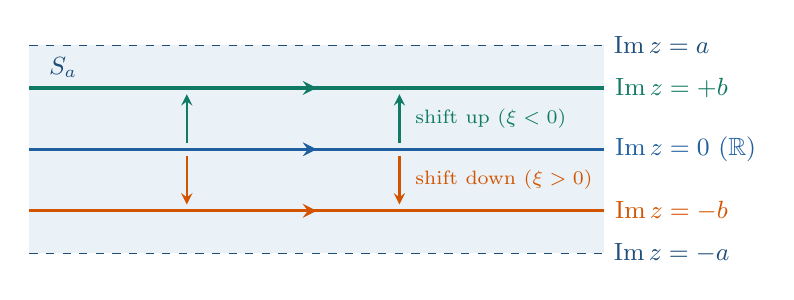
\begin{tikzpicture}[>=stealth,font=\small,
 midarrow/.style={postaction={decorate},decoration={markings,mark=at position .50 with {\arrow{>}}}}]
 % Holomorphic strip S_a
 \fill[lightblue] (-3.65,-1.32) rectangle (3.65,1.32);
 \draw[courseblue,dashed] (-3.65,1.32) -- (3.65,1.32) node[right,text=courseblue] {$\Imag z=a$};
 \draw[courseblue,dashed] (-3.65,-1.32) -- (3.65,-1.32) node[right,text=courseblue] {$\Imag z=-a$};
 \node[text=courseblue] at (-3.22,1.04) {$S_a$};
 % Original contour: real line
 \draw[cayleyblue,very thick,midarrow] (-3.65,0) -- (3.65,0) node[right,text=cayleyblue] {$\Imag z=0$ ($\R$)};
 % Shifted contour up: Im z = +b (for xi < 0)
 \draw[cayleyteal,very thick,midarrow] (-3.65,0.78) -- (3.65,0.78) node[right,text=cayleyteal] {$\Imag z=+b$};
 % Shifted contour down: Im z = -b (for xi > 0)
 \draw[cayleyorange,very thick,midarrow] (-3.65,-0.78) -- (3.65,-0.78) node[right,text=cayleyorange] {$\Imag z=-b$};
 % Vertical shift arrows
 \draw[->,cayleyteal,thick] (-1.65,0.08) -- (-1.65,0.70);
 \draw[->,cayleyteal,thick] (1.05,0.08) -- (1.05,0.70)
  node[midway,right,xshift=2pt,font=\scriptsize,text=cayleyteal] {shift up ($\xi<0$)};
 \draw[->,cayleyorange,thick] (-1.65,-0.08) -- (-1.65,-0.70);
 \draw[->,cayleyorange,thick] (1.05,-0.08) -- (1.05,-0.70)
  node[midway,right,xshift=2pt,font=\scriptsize,text=cayleyorange] {shift down ($\xi>0$)};
\end{tikzpicture}

\vspace{0.15em}
{\small The line of integration $\R$ (blue) can be shifted vertically to any
height $y\in(-a,a)$ inside $S_a$ without changing $\widehat f(\xi)$. Shifting
down to $-b$ for $\xi>0$ (orange) or up to $+b$ for $\xi<0$ (teal) yields
the exponential decay factor $|e^{-2\pi i(x+iy)\xi}|=e^{-2\pi b|\xi|}$.}
\end{minipage}
\end{lecturefigure}

\begin{proof}
For fixed $\xi\in\R$, the function $g(z)=f(z)e^{-2\pi i z\xi}$ is
holomorphic on $S_a$. Take the rectangle with horizontal edges at
heights $0$ and $y$ and vertical edges at $x=\pm R$. By Cauchy's theorem,
the integral around this rectangle vanishes.

\begin{lecturefigure}
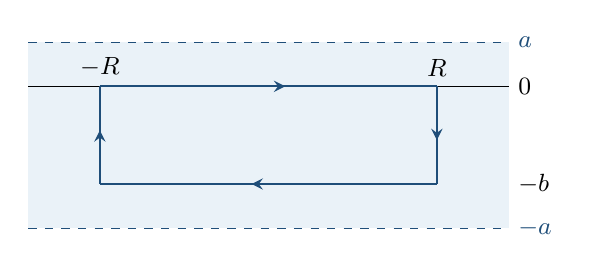
\begin{tikzpicture}[>=stealth,font=\small,
 midarrow/.style={postaction={decorate},decoration={markings,mark=at position .55 with {\arrow{>}}}}]
 \fill[lightblue] (-3.05,-1.28) rectangle (3.05,1.08);
 \draw[courseblue,dashed] (-3.05,1.08) -- (3.05,1.08) node[right] {$a$};
 \draw[courseblue,dashed] (-3.05,-1.28) -- (3.05,-1.28) node[right] {$-a$};
 \draw (-3.05,0.52) -- (3.05,0.52) node[right] {$0$};
 \draw[courseblue,thick,midarrow] (-2.14,0.52) -- (2.14,0.52);
 \draw[courseblue,thick,midarrow] (2.14,0.52) -- (2.14,-0.72);
 \draw[courseblue,thick,midarrow] (2.14,-0.72) -- (-2.14,-0.72);
 \draw[courseblue,thick,midarrow] (-2.14,-0.72) -- (-2.14,0.52);
 \node[above] at (-2.14,0.52) {$-R$}; \node[above] at (2.14,0.52) {$R$};
 \node[right] at (3.05,-0.72) {$-b$};
\end{tikzpicture}

{\small The contour for a shift to $y=-b$.}
\end{lecturefigure}

For $y<0$ (as shown above for $y=-b$), traversing the rectangle clockwise
orients the top edge along $\R$ from left to right and the bottom edge at
height $y$ from right to left:
\[
 \int_{\text{top}} g(z)\,dz
  = \int_{-R}^{R} f(x)e^{-2\pi ix\xi}\,dx,
 \qquad
 \int_{\text{bottom}} g(z)\,dz
  = -\int_{-R}^{R} f(x+iy)e^{-2\pi i(x+iy)\xi}\,dx.
\]
(When $y>0$, the roles of the top and bottom edges reverse, and traversing
counterclockwise produces the same two horizontal integrals with the same
signs.) Cauchy's theorem therefore gives
\[
 \int_{-R}^{R} f(x)e^{-2\pi ix\xi}\,dx
 - \int_{-R}^{R} f(x+iy)e^{-2\pi i(x+iy)\xi}\,dx
 + \int_{\text{vertical edges}} g(z)\,dz = 0.
\]

Along a vertical edge $z=\pm R+it$ between heights $0$ and $y$,
\[
 |g(z)|\leq\frac{A}{1+R^2}e^{2\pi|y\xi|}.
\]
The length of each edge is $|y|$, so both vertical integrals tend to zero
as $R\to\infty$. Both horizontal integrals converge absolutely by
moderate decay, so letting $R\to\infty$ gives \eqref{eq:shift}.

For $\xi>0$ set $y=-b$, and for $\xi<0$ set $y=b$. In either case
$|e^{-2\pi i(x+iy)\xi}|=e^{-2\pi b|\xi|}$. The same bound holds at
$\xi=0$ and for $b=0$ by direct integration on the real axis.
\end{proof}


\section{Fourier inversion}

\begin{theorem}[Fourier inversion on $\mathcal F$]\label{thm:fourier-inversion}
If $f\in\mathcal F$, then for every $x\in\R$,
\[
 f(x)=\int_{-\infty}^{\infty}\widehat f(\xi)e^{2\pi ix\xi}\,d\xi.
\]
The integral on the right converges absolutely.
\end{theorem}
%
%\begin{exercise}[An exponential integral]
%For $A>0$ and $B\in\R$, verify directly that
%$\displaystyle\int_0^\infty e^{-(A+iB)\xi}\,d\xi=(A+iB)^{-1}$.
%\end{exercise}
%
%\begin{proof}[Proof of Theorem~\ref{thm:fourier-inversion}]
%Choose $a>0$ with $f\in\mathcal F_a$ and fix $0<b<a$. By
%Theorem~\ref{thm:shift}, $\widehat f$ is absolutely integrable. Split
%the inverse integral at $\xi=0$. For its positive half, shift the
%Fourier integral to height $-b$:
%\begin{align*}
% \int_0^\infty\!\widehat f(\xi)e^{2\pi ix\xi}\,d\xi
% &=\int_{-\infty}^{\infty} f(u-ib)
%    \left(\int_0^\infty e^{-2\pi i(u-ib-x)\xi}\,d\xi\right)du\\
% &=\frac{1}{2\pi i}\int_{-\infty}^{\infty}
%    \frac{f(u-ib)}{u-ib-x}\,du.
%\end{align*}
%Fubini's theorem applies because the absolute value of the integrand
%in the double integral is bounded by
%$A(1+u^2)^{-1}e^{-2\pi b\xi}$ for $\xi>0$. The inner integral is
%evaluated by the preceding exercise. For the negative half, shift
%to height $+b$ and substitute $\xi=-\eta$ to obtain
%\[
% \int_{-\infty}^0\!\widehat f(\xi)e^{2\pi ix\xi}\,d\xi
% =-\frac{1}{2\pi i}\int_{-\infty}^{\infty}
%    \frac{f(u+ib)}{u+ib-x}\,du.
%\]
%
%For $R>|x|$, close the two horizontal segments at heights $\pm b$
%with vertical sides at $\pm R$. Traverse the lower edge to the right
%and the upper edge to the left.
%
%\begin{lecturefigure}
%\begin{tikzpicture}[>=stealth,font=\small,
% midarrow/.style={postaction={decorate},decoration={markings,mark=at position .62 with {\arrow{>}}}}]
% \fill[lightblue] (-2.8,-0.68) rectangle (2.8,0.68);
% \draw[densely dotted] (-2.95,0) -- (2.95,0);
% \draw[courseblue,thick,midarrow] (-2.8,-0.68) -- (2.8,-0.68);
% \draw[courseblue,thick,midarrow] (2.8,-0.68) -- (2.8,0.68);
% \draw[courseblue,thick,midarrow] (2.8,0.68) -- (-2.8,0.68);
% \draw[courseblue,thick,midarrow] (-2.8,0.68) -- (-2.8,-0.68);
% \node[right] at (2.8,0.68) {$\Imag z=b$};
% \node[right] at (2.8,-0.68) {$\Imag z=-b$};
% \fill (0.65,0) circle (1.3pt) node[above] {$x$};
%\end{tikzpicture}
%\end{lecturefigure}
%
%The residue of $f(z)/(z-x)$ at $x$ is
%$f(x)$, so its integral around the rectangle equals $2\pi i f(x)$.
%On either vertical side, the integrand is bounded by
%$A/((1+R^2)(R-|x|))$, and the length is $2b$. Letting $R\to\infty$
%leaves exactly the two horizontal integrals above, with the stated
%signs. Their sum gives $f(x)$.
%\end{proof}

%\begin{remark}[From integrals to sums]
%The same contour shift will be used in the next lecture to prove
%Poisson summation, $\sum_{n\in\Z} f(n)=\sum_{n\in\Z}\widehat f(n)$.
%\end{remark}

\end{document}
